\documentclass[../main.tex]{subfiles}

\begin{document}

\section{Anodes (Mike/Chao/Arihant/Rana)}
% Overall deadline: 18th December to hand over to Co-Is.
% Suggested CoIs: split between Harry, Denis and Chris (as discussed 16th December)
% All three: please review 3.1 introduction and 3.4 outlook
% Harry: 3.2 bulk properties (authored by Mike, with contributions from Rana in 3.2.1 and 3.2.4)
% Denis: 3.3 graphite surfaces and interfaces except 3.3.4 (authored by Chao, with contributions from Rana in 3.3.1) 
% Chris: 3.3.4: the solid liquid interface (this could also be a separate subsection 3.4). Authored by Arihant. Note: Arihant has done first draft of SEI (8th Jan: Mike has reviewed, structural rearragnement to be discussed). As last author, we feel CS should also be familiar with the other contents in the section.
% Mike and Lucy have proof-read the entire section.
% All welcome to review other subsections if they find time, but should prioritise the above so everything is reviewed. We suggest permuting the three CoIs between the subsections on the next iteration of editing. 
% An additional figure/description on Frenkel, vacancy mechanisms in 3.2.4 (which can be additionally cross-referenced in cathodes) is also pending, overview discussed and to be finished (17th/18th) but the postdocs consider the section otherwise complete. 

% Surface stabilisation mechanisms in graphite to be added (discussed Rana/Chao).

\subsection{Introduction and historical context (Mike)}
\label{sec:anodes_intro}
% - Mike: I have taken the lead on this part in exchange for others hopefully helping on the anode bulk part. This section will be of broad interest to everyone working on anodes and possibly everyone in the review, since it talks about the electrolyte and briefly the cathode as well. So when I'm done, we should take turns improving it.
% November 27th

 Critical to the success of lithium-ion batteries was the development of graphite-based anodes. Graphite proved to be ideal for this application due to its low (de)-intercalation potential, only slightly higher than that of metallic lithium, and high theoretical gravimetric capacity of 372 mAh/g. However, many key degradation mechanisms in present day Li-ion batteries that lead to their eventual failure, including cracking/reformation of the solid electrolyte interphase (SEI) and lithium plating, are still intimately connected with graphite-based anodes \cite{VETTER2005269,ma6041310}. The understanding of these mechanisms is still far from complete and leads to complex, non-linear degradation behaviour that is difficult to predict \cite{YANG201728}, motivating the development of multiscale models with a descriptive and predictive capability (see also: reviews on parameterisation and continuum modelling in the same special issue). A critical starting point for these models is a physically accurate atomistic description of the graphite and its interface with organic electrolytes. 

The possibility to form lithium-graphite intercalation compounds, also known as ``stages'', up to a stoichiometry of LiC$_{6}$ was known in 1975, albeit at that time it was only possible to form them by heat treating powders \cite{GUERARD1975337,Woo1983,BASU1979275}. Initial attempts to intercalate lithium into graphite electrochemically resulted in co-intercalation of the organic solvent and exfoliation of the graphite \cite{BESENHARD1976111}. In 1983, \citeauthor{yazami1983} reported the first successful intercalation into graphite using a solid polymer electrolyte \cite{yazami1983}. \citeauthor{Fong1990} found that reversible lithium intercalation could be achieved in liquid organic electrolytes using ethylene carbonate (EC) as part of the solvent, which finally enabled the formation of a stable SEI on the graphite surface \cite{Fong1990}. Mixtures of EC and dimethyl carbonate (DMC) were developed by \citeauthor{TARASCON19931221} in 1993 \cite{TARASCON19931221} and present day graphite-based Li-ion batteries are still primarily based on this electrolyte mixture. The key challenge was finding a solvent chemistry that provided sufficient ionic conductivity, did not decompose significantly at the $\sim$4 V cathode potential, while also avoiding co-intercalatation into the graphite and producing a stable SEI on its surface. Further incremental improvements in performance have since been achieved through additional additives, and more recently the inclusion of small amounts of silicon in the anode as a secondary material. However, this section focuses entirely on graphite since it remains the primary anode electrode material in the majority of commercial lithium-ion cells \cite{asenbauer_success_2020}.

Here, the experimentally confirmed Li-graphite stages and the nomenclature necessary for atomistic models of bulk behaviour are defined. Atomistic modelling in the graphite bulk is outlined, including both thermodynamic and kinetic properties. The key graphite surfaces relevant to understanding the initial intercalation are described, then moving to modelling at the graphite edges and the interface with the electrolyte. Throughout, it is shown how these models enable quantitative understanding of the physical mechanisms of Li intercalation in the graphite bulk, the initial insertion at the graphite edges, and the interface between graphite and the electrolyte. Along the way the key experimentally observable parameters are outlined, showing success stories of atomistic models to not only quantify and describe those parameters but also to predict new behaviour. In some cases, quantitative disagreement between model and experimental observations is also informative and can create new research directions. Lastly, work linking atomistic and continuum models is presented in the case of the technologically important solid electrolyte interphase (SEI). In the outlook, key remaining challenges are presented for modelling not only graphite, but also next generation materials such as silicides.  

\subsection{Bulk Properties}
\label{sec:anode_bulk}
% Mike + incorporated parts from Rana.

\subsubsection{Graphite structure and Li-graphite stages}
\label{sec:anodes_structure_stages}

Graphite possesses a layered structure with carbon atoms forming a network of hexagons in each layer. The carbon atoms located within one layer are covalently bonded to each other, whereas the weak interlayer binding arises from the dispersion or van der Waals (vdW) interactions \cite{GUERARD1975337,PhysRevLett.50.182,persson2010,Woo1983,Dahn1991,hazrati_li_2014,Konar2015}. The lowest energy stacking of the carbon layers is AB stacked (Figure~\ref{fig:graphite_stages_schematics}b), but synthesised graphite structures also contain a small amount of rhombohedral (ABC-stacked) domains \cite{Shi_1996}. 

Li-graphite stages, also known as Li-graphite intercalation compounds (Li-GICs), are lithium-concentration dependent structures of various stoichiometries \cite{Woo1983,GUERARD1975337,Konar2015,Sethuraman2010,Dahn1991}. In Li-GICs, Li atoms form a 2D hexagonal ($\sqrt{3} \times \sqrt{3}$)R 30$^{\circ}$ superstructure with Li atoms sitting directly above each other, as shown in Figure~\ref{fig:graphite_stages_schematics}a. The stage number, $n$, denotes the number of graphene layers between each lithium-filled layer \cite{Dahn1991,Ohzuku1993,Konar2015,GUERARD1975337}.
The experimentally confirmed stages adopt different stackings in the carbon host lattice, as shown in Figure~\ref{fig:graphite_stages_schematics}. The standard nomenclature for GICs \cite{PhysRevLett.50.182} denotes the carbon stacking and Li occupancies: periodic carbon layer stackings along the [001] axis are designated by uppercase letters separated by Greek lowercase letters if Li is intercalated between planes. For instance, fully lithiated Stage I LiC$_{6}$ ($x=1$) adopts A$\alpha$A$\alpha$A$\alpha$ stacking \cite{Konar2015,He_2013,YAZAMI2006312}. Here $\alpha$ denotes a lithium filled layer and $x$ is the fraction of Li in Li$_{x}$C$_{6}$ ($0 \leq x \leq 1$).

\begin{figure}[h!]
    \begin{center}
    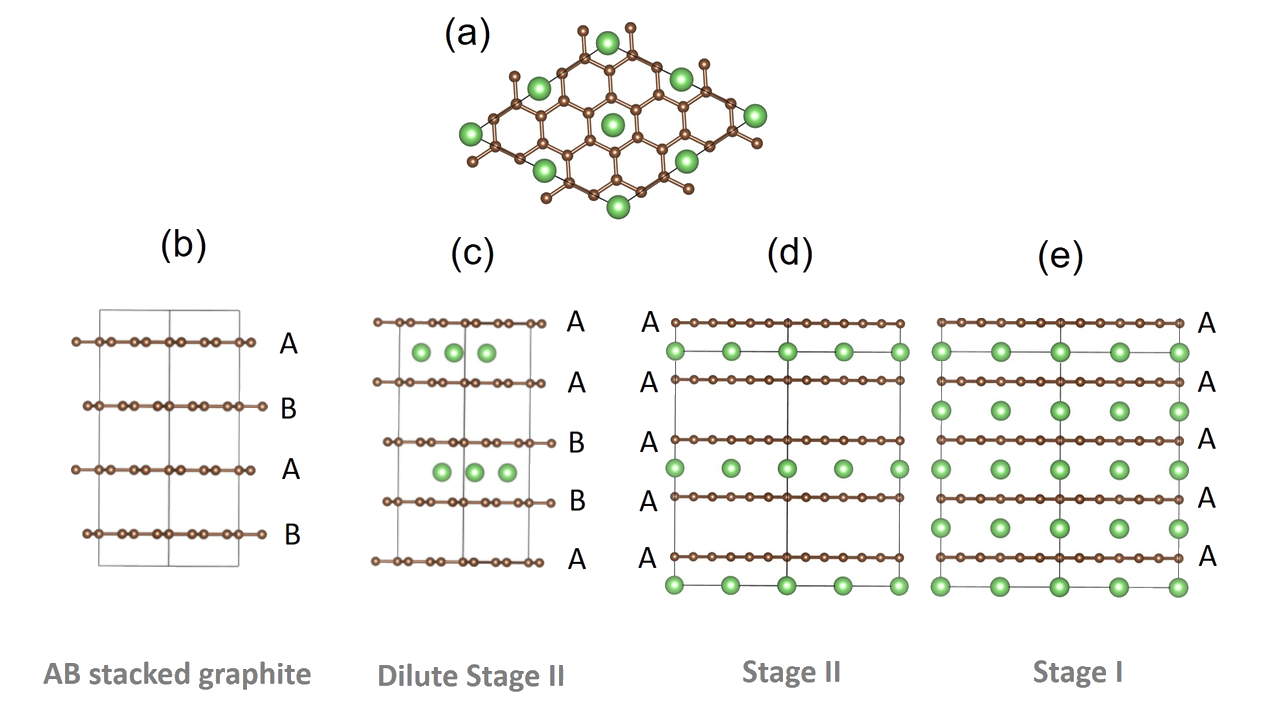
\includegraphics[width=0.98\columnwidth]{figures/stages_version4}
    \caption{{{Structural representations of different carbon stackings in
    experimentally confirmed stages of graphite. (a) Top down view of carbon
    and lithium arrangements in Stages I and II. (b-e): side views, showing
    the layers occupied with Li and carbon stackings in (b) empty AB stacked
    graphite, (c)~A\(\alpha\)AB\(\beta\)B stacked dilute
    Stage II, with~\(\beta\) indicating a lithium layer translated
    with respect to~\(\alpha\), (d)
    A\(\alpha\)AA\(\alpha\)A Stage II and (e)~
    A\(\alpha\) stacked Stage I}{. Green represent Li atoms while
    the brown indicate C atoms. Reproduced from ref. \cite{Mercer2021}}
    {\label{fig:graphite_stages_schematics}}%
    }}
    \end{center}
\end{figure}

Li-GICs vary not only in their lithium concentrations, but also in their carbon stackings. The current concensus of all known stages, their carbon stackings and their lithium stoichiometries, is tabulated in Table~\ref{table:graphite_stages}.

\begin{table}
    \caption{{Overview of carbon stackings and stoichiometries of lithium-graphite stages from the literature, where Latin characters denote carbon stackings and Greek characters denote Li-filled layers. \cite{TRUCANO1975,Okamoto1989,GUERARD1975337,Billaud1996,BILLAUD2002299,PhysRevLett.50.182,Dahn1991,Ohzuku1993}}}
    \label{table:graphite_stages}
    \begin{tabular}{|c c c|} 
         \hline
         Stage & Stacking & $x$ in Li$_{x}$C$_{6}$  \\
         \hline
         Stage I & A$\alpha$A$\alpha$ & $x = 1$ (LiC$_{6}$)    \\
         Stage II & A$\alpha$AA$\alpha$A & $x = 0.5$ (LiC$_{12}$)  \\
         Dilute Stage II (IID) & A$\alpha$AB$\beta$B & $x \approx 0.33$ (LiC$_{18}$)   \\
         Stage III & A$\alpha$AB/A$\alpha$ABA$\alpha$AC & $x \approx 0.22$ (LiC$_{27}$) \\
         Stage IV & Unknown & $x \approx 0.17$ (LiC$_{36}$)  \\
         Dilute Stage I (ID) & AB & $x \approx 0.083$ (LiC$_{72}$)  \\
         Graphite & AB & $x = 0$   \\
         \hline
    \end{tabular}
\end{table}

Experimental observation of these stages relies largely on probing the average interlayer carbon spacing through diffraction measurements. Probing the lithium orderings of Li-GICs through experimental techniques remains very difficult \cite{Zheng1995,Konar2015,Senyshyn2013,Taminato2016,Mercer2019,Mercer2021}, but as shown in section~\ref{sec:anodes_entropy}, atomistic techniques shed light on these orderings.

Thermodynamic and kinetic properties of Li-GICs have been studied by considering various structures of LiC$_{6n}$ using \textit{First Principles} DFT \cite{RanaLiC6, Hakim, Qiong, Doreen,JI201866,Wang,persson2010,persson2010lithium,hazrati_li_2014,peng2020lithium,hazrati_li_2014}, mean field \cite{Mercer2019,Leiva2017b,OTERO2017569}, canonical and grand canonical Monte Carlo, \cite{Gavil_n_Arriazu_2018,persson2010,C7CP04253A}, and kinetic Monte Carlo simulation techniques \cite{JI201866,persson2010,gavilan-arriazu_effect_2020,gavilan-arriazu_kinetic_2020,GAVILANARRIAZU2018133}. The rest of the section outlines \textit{First Principles} studies of experimentally measurable bulk thermodynamic properties before describing atomistic modelling of kinetic properties.

\subsubsection{Equilibrium potential and measured open circuit voltage (OCV)}
\label{sec:anodes_ocv}
%- lead: Mike
%- review: Denis
Knowledge of the correct phase behaviour of an intercalation electrode is an important pre-requisite to building a dynamic model of the intercalation process. One of the most directly measurable observables is the experimental open circuit voltage (OCV), which is related to the equilibrium potential determinable from atomistic methods (c.f. methods section~\ref{sec:properties_equilibriumvoltage}). The OCV is an important input parameter in continuum models, and is also used in control models, for example, to determine the state of charge of a battery within a Battery Management System (BMS) \cite{PLETT2004262}. Inputting a polynomial fit to the experimental OCV at an arbitrary temperature without physical meaning could lead to incorrect predictions of temperature-dependent behaviour in these models. Therefore, to attain predictive, dynamic, models on longer length scales, atomistic models of the OCV and equilibrium potential are important, and can contribute to physically more robust and more predictive temperature dependence in continuum and control models \cite{VanderVen2020,Urban2016}.

In any intercalation electrode, ordered phases give rise to steps in the OCV. In the lithium-graphite system, the ordered stages described in section~\ref{sec:anodes_structure_stages} therefore give rise to characteristic features in OCV versus $x$ curves \cite{Dahn1991,Ohzuku1993} as shown in in Figure~\ref{fig:expt_ocv}.  The influence of the Li-graphite stages on the measured OCV at $T \approx 25$ $^{\circ}$C has been well characterised \cite{Sole2014,Zheng1995,Senyshyn2013,Taminato2016,Allart2018,Sethuraman2010,Markevich2005,Dahn1991,Ohzuku1993}, although a more thorough study of the temperature dependence of the OCV has only been conducted more recently \cite{Mercer2021}. Each OCV plateau represents a different two phase equilibrium. At zero Kelvin, there is no contribution from configurational entropy and each step represents a sudden transition between two different two phase equilibria. This is the behaviour that can be captured by using DFT codes. The cluster expansion framework, described in more detail in methods section~\ref{sec:cluster_expansion}, allows the accuracy of DFT to be retained to explore configurational degrees of freedom. Thermal fluctuations can be included by determining effective cluster interactions (ECIs) from fitting DFT data and using these as parameters within a Monte Carlo method (section~\ref{sec:monte_carlo}). The entropy contribution at temperature, $T> 0$ K has the effect of smoothing out those steps \cite{Mercer2019,OTERO2017569,REYNIER2003850,Mercer2021}, which is caused by some limited single phase solubility around the stoichiometric composition. This can be seen in experimentally measured OCV profiles at $T \approx 300$ K, such as the ones shown in in Figure~\ref{fig:expt_ocv}.  

    \begin{figure}
    \centering
    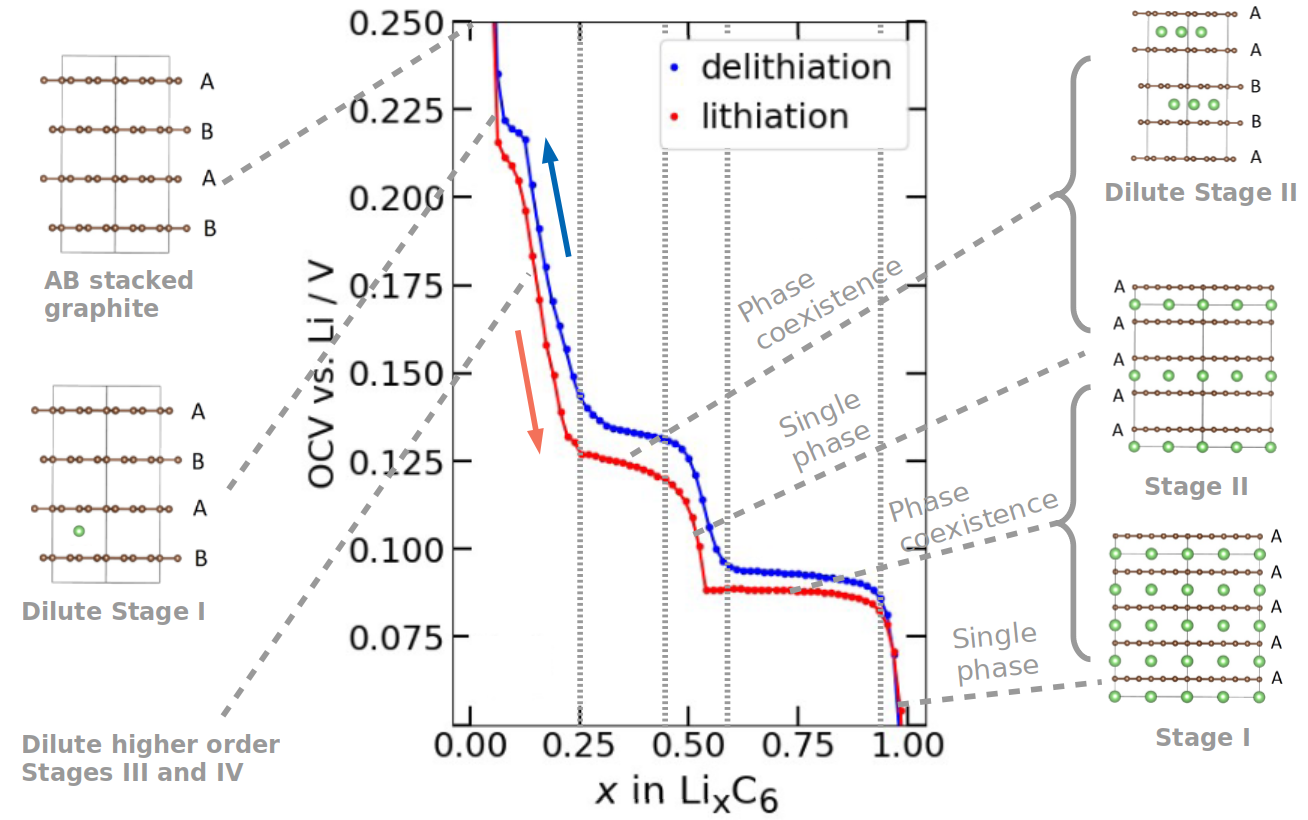
\includegraphics[scale=1.2]{figures/ocv_and_stages.png}
    \caption{Illustration of OCV features of lithium in graphite using experimental data from ref. \citenum{Mercer2019}. Lithiation and delithiation behaviour is overlaid; labelled stages are linked to the lithiation profile, which is closer to the true equilibrium potential. Reproduced from Ref. \citenum{Mercer2021}}
    \label{fig:expt_ocv}
\end{figure}

The equilibrium potential versus $x$ can be modelled through atomistic techniques. For example, Li-graphite phase diagrams were constructed and the equilibrium potential was modelled by \citeauthor{persson2010} \cite{persson2010}. They performed a cluster expansion of Li degrees of freedom from total energy DFT calculations (c.f. methods, section~\ref{sec:cluster_expansion}), by fixing the carbon stacking degrees of freedom. Those degrees of freedom represent the host lattice stackings in the experimentally confirmed stages shown in Figure~\ref{fig:graphite_stages_schematics}. Typically, different cluster expansions are performed in Li-vacancy lattices of the respective hosts \cite{persson2010,hazrati_li_2014,Mercer2021}, to account for carbon stacking degrees of freedom with the result from a more recent work \cite{Mercer2021} represented in Figure~\ref{fig:persson_graphitephases}a. Within this work, AA, AABB, and AB stackings of the host lattice were considered, representing all stages of order up to II (c.f. Figure~\ref{fig:graphite_stages_schematics}). Reference states at $x=0$ and $x=1$ were used in AB and AA stackings, respectively, to linearly correct the free energy and thus obtain the formation energies at each lithium concentration. The convex hull over all stackings represents the lowest energy structure for a given $x$ value. A common tangent construction between the different stackings represents two phase coexistence. The slope of the resultant ground state free energy profile, $dG(x)/dx$, (equation~\ref{eq:chemicalpotgibbs}) equals the intercalated Li chemical potential, $\mu$, and therefore minus the equilibrium potential at $T=0$ K, as represented more generally in Figure~\ref{fig:vanderven_thermodynamics} and the surrounding discussion in the Methods section. 

The phase behaviour of the lithium-graphite system, and therefore the voltage profile, is sensitive to the van der Waals (vdW) interactions between the carbon planes \cite{RanaLiC6, Hakim,persson2010}.
Conventional DFT approaches without accounting for vdW interactions do not correctly reproduce the structure and energetics of graphite and Li-GICs \cite{RanaLiC6, Hakim,persson2010} (Figure~\ref{fig:persson_graphitephases}b). Therefore, vdW-corrected DFT approaches, for example DFT-D2 \cite{Grimme-1} and DFT-D3 \cite{Grimme-3}, are important for correctly describing the phase behaviour and dynamics of graphite and Li-GICs. \citeauthor{persson2010} considered the van der Waals interaction as a constant \cite{persson2010}. This approximation can accurately describe the step height at $x=0.5$ (the height difference represents the difference between the chemical potentials in the Stage I-Stage II and Stage II-Stage IID coexistence regions). The simulated voltage profile Figure~\ref{fig:persson_graphitephases}b (blue line), shows that the constant vdW interaction results in a systematic error in the voltage scale.

Voltage profiles like the ones shown in Figure~\ref{fig:persson_graphitephases}b represent the ground state behaviour, at $T = 0$ K. As an additional step, cluster expansions can be used to parameterise a Monte Carlo simulation (methods section~\ref{sec:monte_carlo}) and therefore include thermal fluctuations. The lithium-graphite phase diagram, Figure~\ref{fig:persson_graphitephases}c has been constructed, by performing a combination of canonical and grand canonical Monte Carlo simulations at different temperatures \cite{persson2010}. 

\begin{figure}
    \centering
    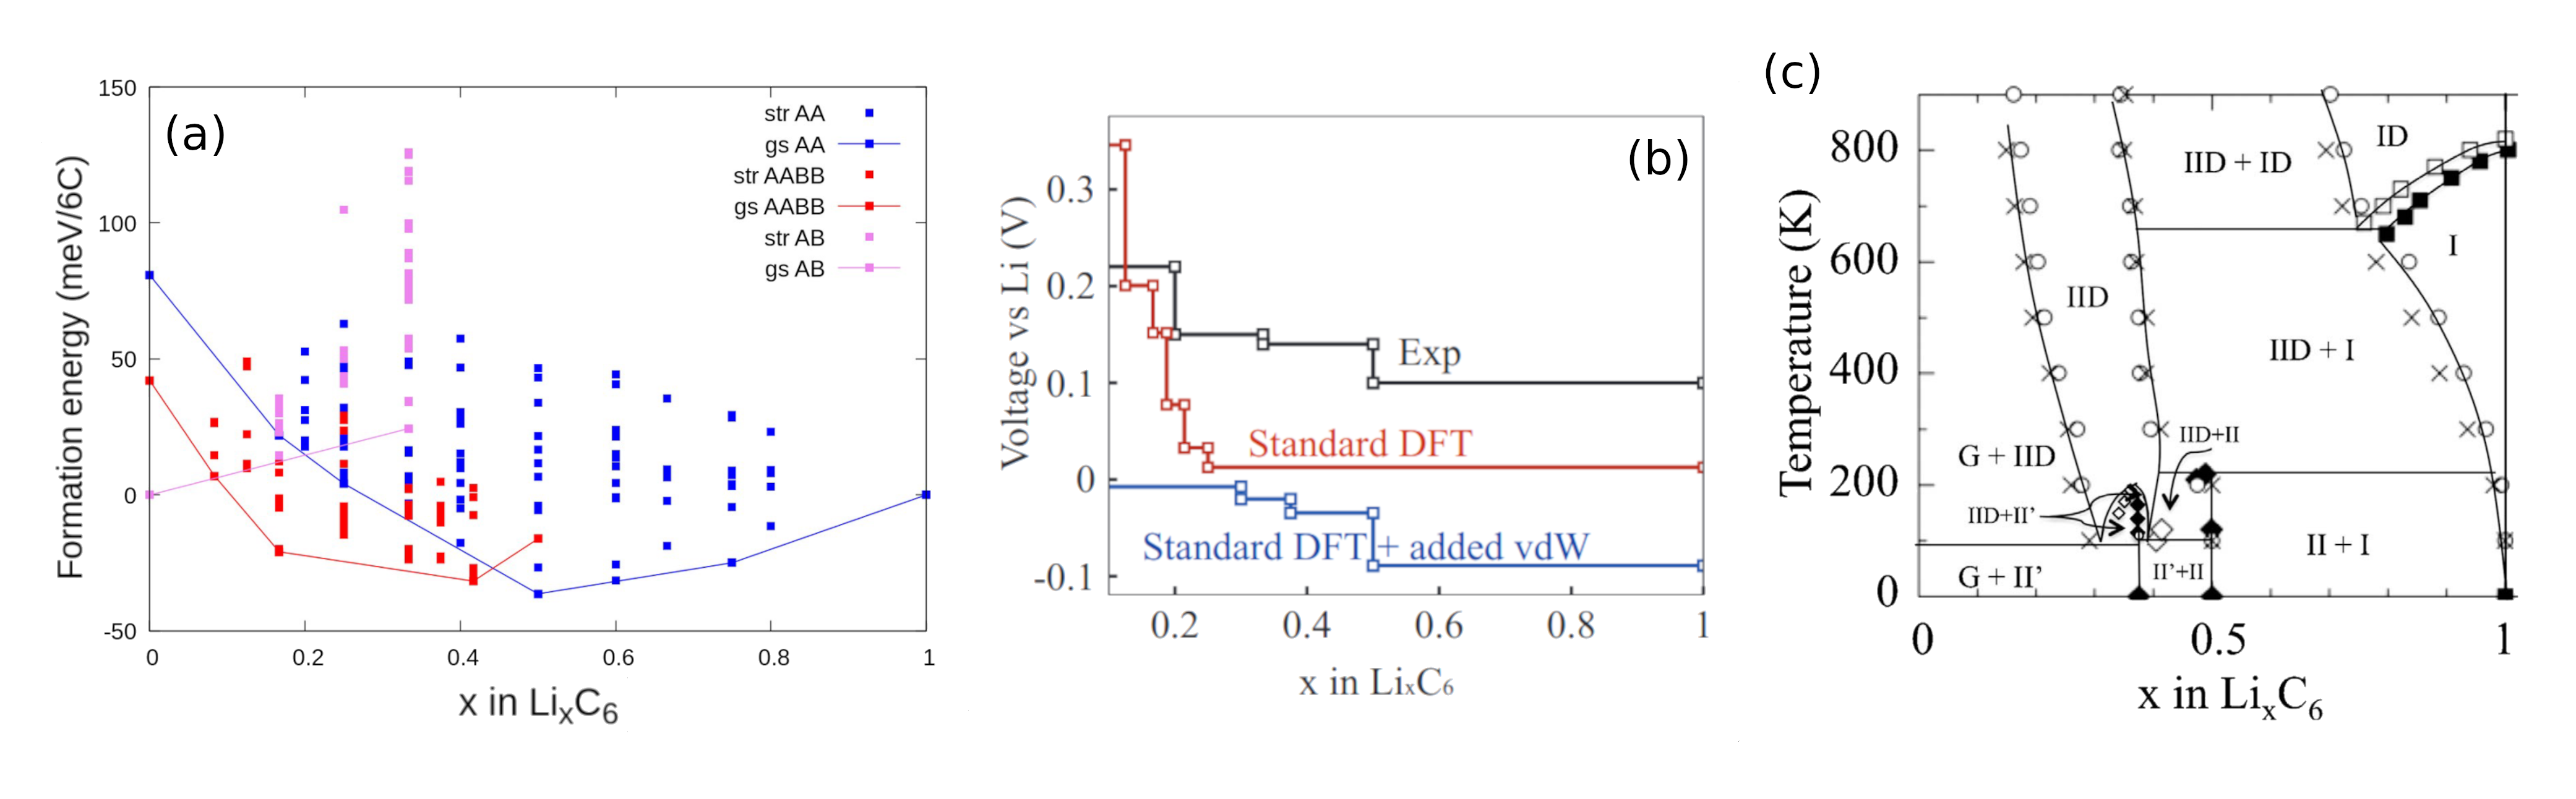
\includegraphics[scale=0.45]{figures/cluster_expansions_persson.png}
    \caption{(a) Formation energies of lithium in graphite performed with different carbon stackings. All calculated structures are denoted ``str'' while the ``gs'' represent the ground state structures in each of the three carbon stackings: AB, AABB, AA. (b) Phase diagram of lithium in graphite, determined by performing Monte Carlo calculations parameterised by effective cluster interactions from DFT calculations. (c) zero kelvin equilibrium potential profiles dependent on different levels of van der Waals corrections. From ref. \citenum{persson2010}}
    \label{fig:persson_graphitephases}
\end{figure}

The experimental OCV and the theoretical equilibrium potential are often, erroneously, considered equivalent. However, the OCV refers to the measured cell voltage without any external current and drifts with time. With sufficient time, it is often assumed the OCV will eventually relax to the equilibrium potential, but meta-stable states can occur that show no variation over experimental time scales of hours or even days.\cite{Liu2014,orisaka2013,Mercer2021} The true equilibrium potential, as defined in equation~\ref{eq:chemicalpotgibbs}, is a thermodynamic quantity and is not history dependent \cite{VanderVen2020,Mercer2021}. Experimentally, a hysteresis of the measureable OCV between lithiation and delithiation is observed for Li/graphite half cells \cite{Ohzuku1993,Zheng1995,Dahn1991,Allart2018,Gallagher2012,YAZAMI2006312,GRIMSMANN201817,didier2020,Mercer2021} as shown in Figure~\ref{fig:expt_ocv}. Hysteresis is observed even after several hours of relaxation time and for $T>298$ K, clearly demonstrating that the measured OCV is not a simple function of the thermodynamic ground state. Hysteresis therefore poses an interesting challenge to atomistic modellers.

It was recently shown that lithiation/delithiation hysteresis in graphite is intimately connected with disorder in Stage II configurations and appears to be associated with a different carbon stacking pathway in each cycling direction \cite{Mercer2021}. Notably, energetic barriers to translate between ground state configurations, as determined through climbing image nudged elastic band (CI-NEB) calculations (methods section~\ref{sec:methods_neb}), do not explain the hysteresis in graphite. Non-ground state configurations are involved in the delithiation direction. Understanding that behaviour requires quantifying the configurational entropy of Li/vacancy arrangements. This approach is explained in more detail in the next section.  

\subsubsection{Entropy (Mike)}
\label{sec:anodes_entropy}
% thermodynamics: 18th December deadline 
-lead: Mike

The internal energy of intercalation electrodes arises largely from electrostatic interactions between the constituents. Those interactions can be well approximated by DFT, c.f. section~\ref{sec:dft}. An atomistic description of the the entropy behaviour of intercalation electrodes, $S(x)$, is also needed to correctly model thermal behaviour at $T>0$ K. The partial molar entropy, $dS(x)/dx$, is an experimentally accessible quantity, which can be probed by monitoring how the OCV, described in the previous section, varies with temperature (equation~\ref{eq:entropy_measurement}, c.f. refs. \citenum{Mercer2019,schlueter_quantifying_2018,Reynier2004,Yazami_2006,THOMAS2003844,OSSWALD2015270} for further details). $S(x)$ is a sum of configurational, vibrational, and electronic components \cite{REYNIER2003850,Reynier2004}. For lithium in graphite, the electronic component can be neglected, and the vibrational component can be well approximated by assigning a Debye temperature to all of the vibrational modes \cite{REYNIER2003850,Reynier2004}, or by computing phonon spectra from \textit{First Principles} \cite{hazrati_li_2014} (c.f. section~\ref{sec:thermal_electronic_vibrational}). The quantity that shows the greatest difference with lithium concentration, $x$, is the configurational entropy of Li/vacancy arrangements, $S_{\rm{config}}$. Because of the staging phenomena described in section~\ref{sec:anodes_structure_stages}, $S_{\rm{config}}$ strongly deviates from ideal solid solution behaviour for Li in graphite.

The partial molar entropy $dS(x)/dx$ is difficult to interpret atomistically, and so integration is required to get $S_{\rm{config}}$,

\begin{equation}
    \int_{x'=0}^{x'=x} \left(\frac{{\partial}S_{\rm{config}}(x')}{{\partial}x'}\right)dx' = S_{\rm{config}}(x) \approx S(x) - S_{\rm{vib}}(x),
    \label{eq:entropy_integration}
\end{equation}

where $S_{\rm{vib}}$ is the vibrational entropy approximated by Debye temperatures  \cite{REYNIER2003850,Reynier2004}. The integration constant is $S_{\rm{config}} = 0$ at $x=0$, because there can be no Li disorder in pure graphite. 

\begin{figure}
    \centering
    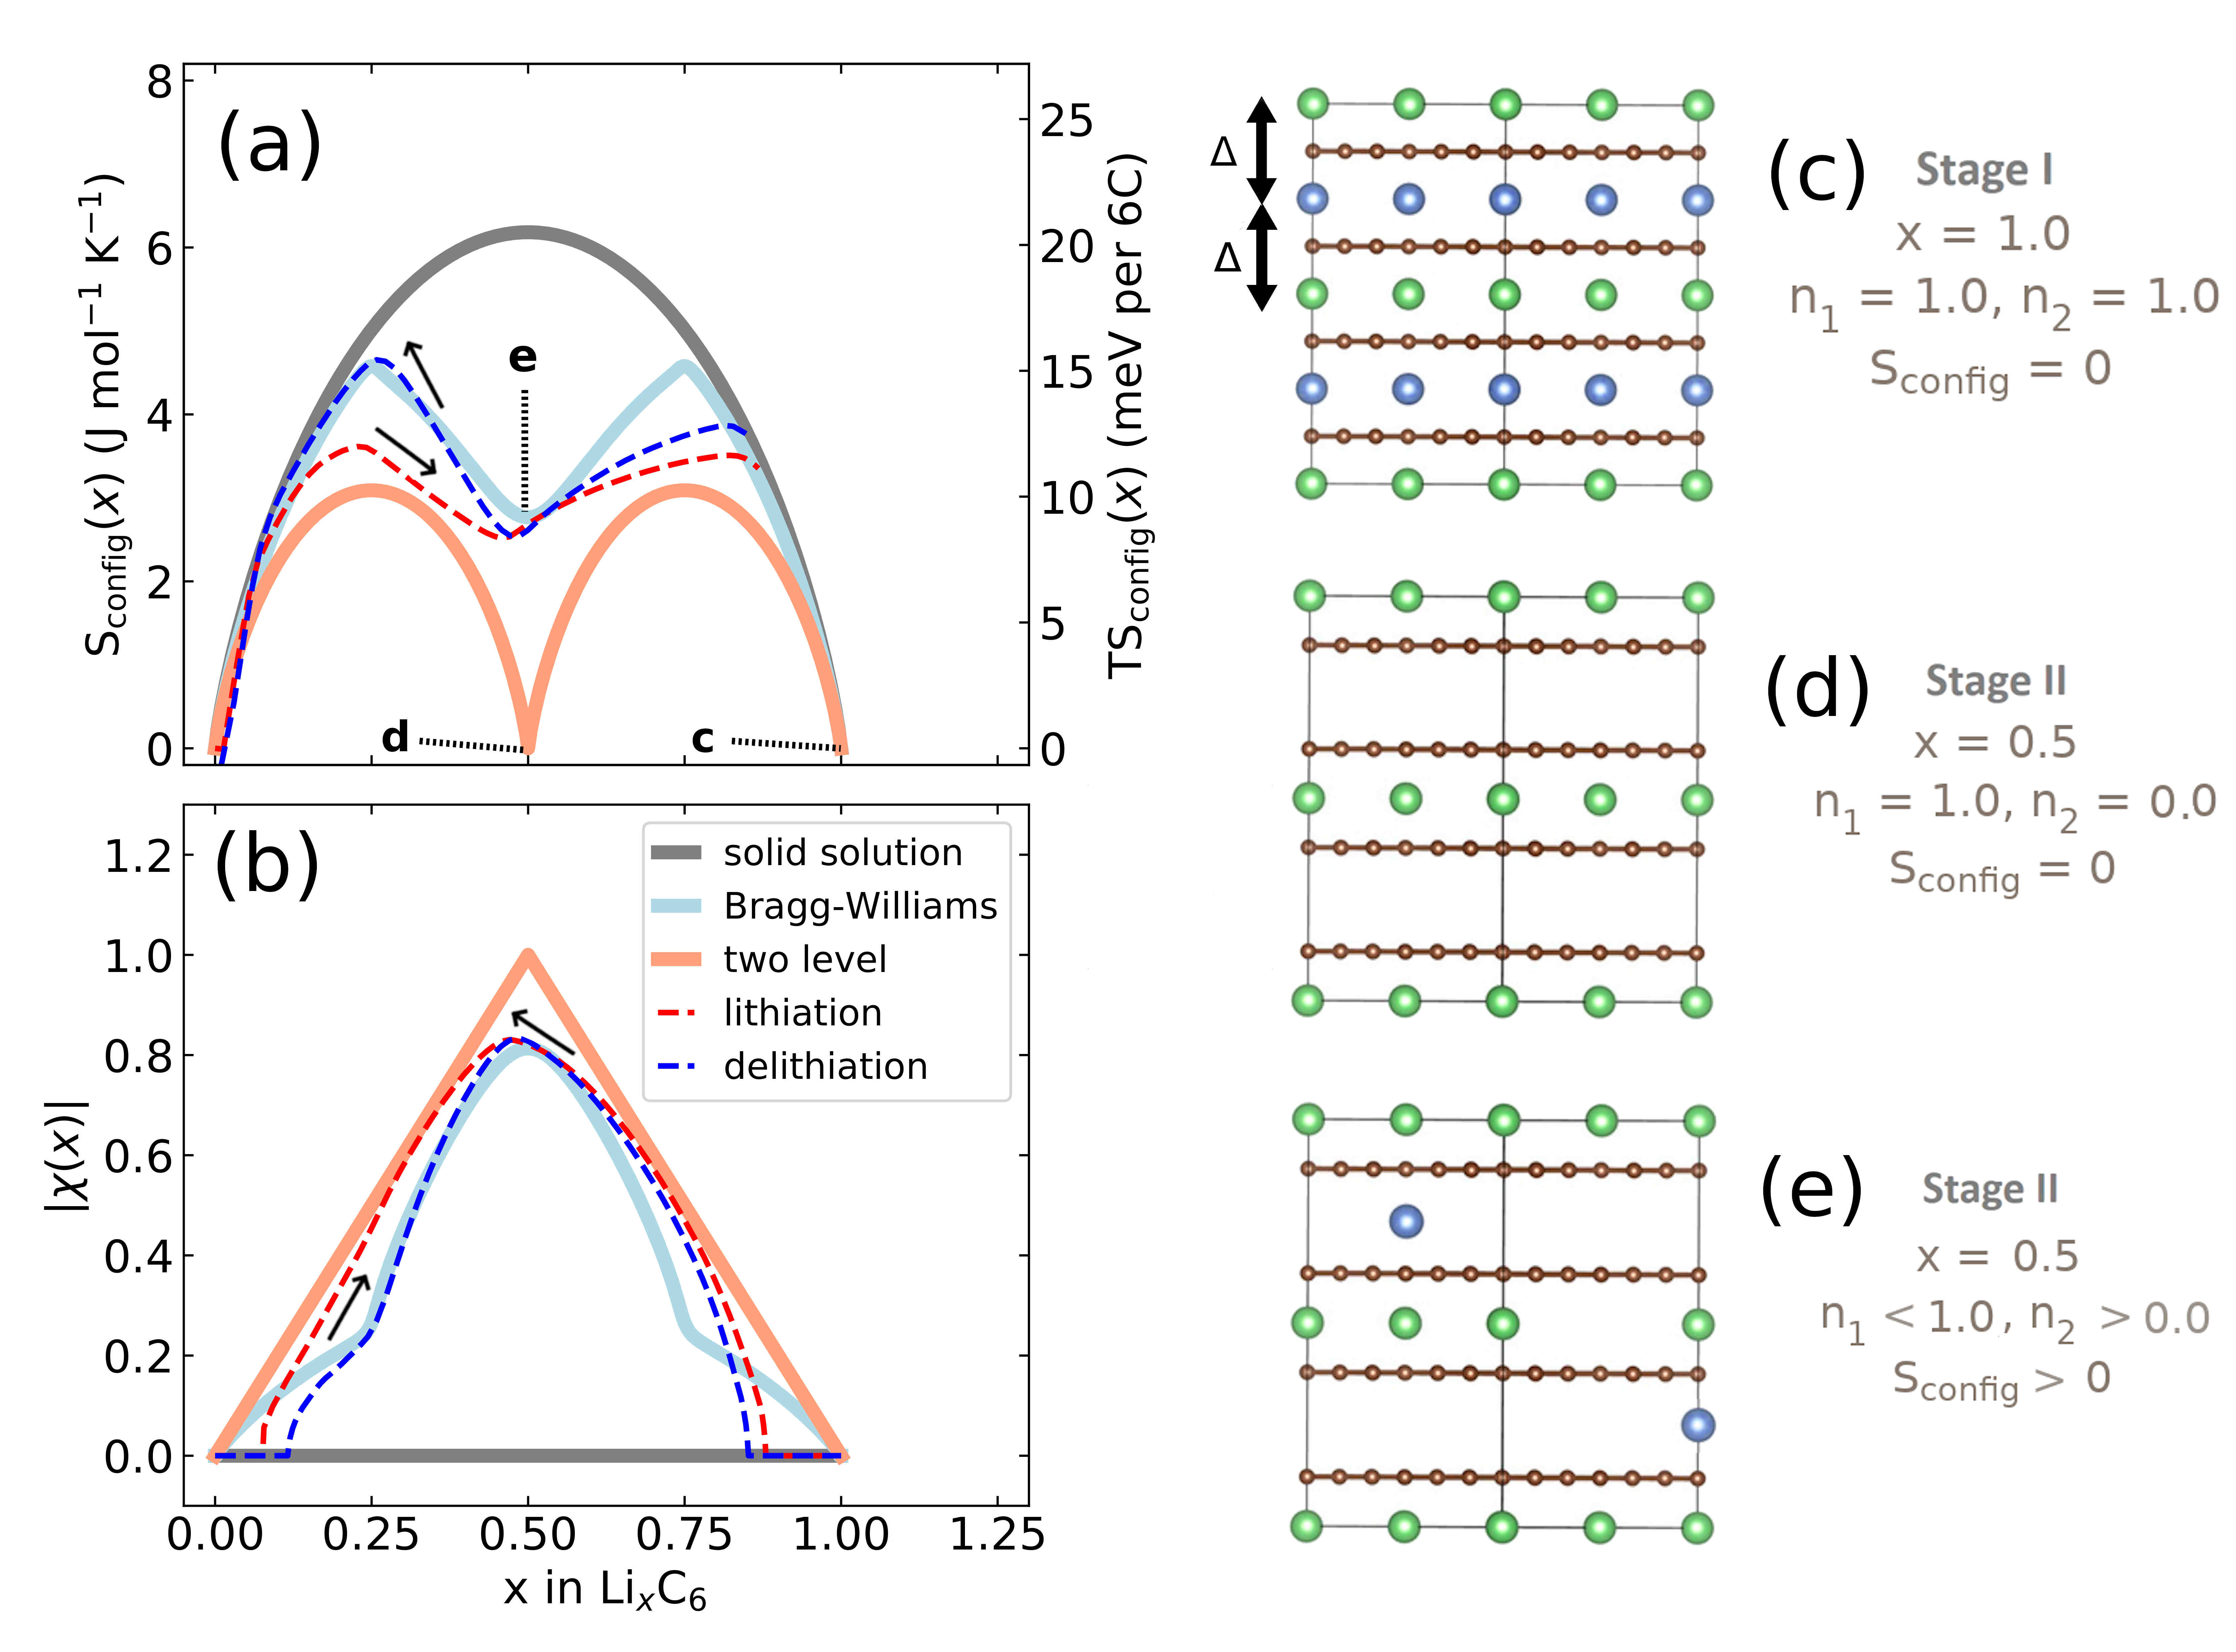
\includegraphics[scale=0.36]{figures/order_parameter_scheme_v2.jpg}
    \caption{(a) Configurational entropy obtained at $T$ = 320 K:~\emph{dark grey solid line}: ideal solid solution;~\emph{light blue solid line}: Bragg-Williams solution;~\emph{orange solid line}: sequential two level solid solution;~\emph{red dashed line}: experimental lithiation;~\emph{blue dashed line}: experimental delithiation. (b) Order parameter \textbar{}\(\chi\)\textbar{}, as described in the main text, labelled as in (a). In (a), select points (c-e) are indicated and schematic representations of the lattice occupations of Li in levels $n_{1}$ (green balls) and $n_{2}$ (blue balls) are shown on the right.}
    \label{fig:entropy_scheme}
\end{figure}

Dashed lines in Figure~\ref{fig:entropy_scheme}a denote post-processed experimental data obtained during lithiation and delithiation using equation~\ref{eq:entropy_integration} from ref. \citenum{Mercer2021}. Qualitatively, this shows more configurational Li disorder, i.e. larger entropy, is obtained during delithiation than lithiation. The lithium arrangements can be split into sublattice occupancies $n_{1}$ and $n_{2}$ arranged in alternate planes as shown visually in Figure~\ref{fig:entropy_scheme}c-e, to assist interpretation. Each sublattice occupancy is linked to the degree of lithiation, $x$, via $x = (n_{1} + n_{2})/2$.

Solid lines in Figure~\ref{fig:entropy_scheme}a-b indicate three hypothetical cases. The orange solid line denotes solid solution (random) filling of Li into one of the sublattices for $x<0.5$, followed by solid solution filling of the other sublattice, resulting in two maxima. Note that $S_{\rm{config}}$ is zero in Stage II at $x=0.5$ (c.f. Figure~\ref{fig:entropy_scheme}d). The dark grey line shows the result for an ideal solid solution, if Li were to fill all available sites at random, i.e. $n_{1} = n_{2}$ for all $x$. The blue solid line is the solution to a Bragg-Williams model \cite{Mercer2019,OTERO2017569} assuming only nearest neighbour repulsive pairwise lithium interactions between planes of $\Delta = 75$ meV and no in-plane interactions. That model allows a direct evaluation of the partition function (c.f. equation~\ref{eq:partition_fn}) by enumerating through all possible arrangements of Li atoms on the two sublattices for a given $x$ within the canonical ensemble. The out-of-plane Li-Li interactions are treated within a mean field (non-local) approximation to simplify the computation (details and formulae in refs. \citenum{Leiva2017b,Mercer2019,OTERO2017569}).

The Bragg-Williams model produces a behaviour in $S_{\rm{config}}(x)$ between that expected for the solid solution and sequential two level filling. At $x=1$, there is a net repulsion on each Li atom of 2$\Delta$, as represented in Figure~\ref{fig:entropy_scheme}c. At $x = 0.5$, one of the sublattices becomes preferentially filled, as represented schematically in Figure~\ref{fig:entropy_scheme}e. In contrast, a perfect Stage II structure as predicted by sequential two level filling (Figure~\ref{fig:entropy_scheme}d) would result in $S_{\rm{config}}(0.5) = 0$. 

These results can be understood within the framework of order parameters \cite{natarajan2017}. The relevant staging order parameter, $\chi(x) = n_{1} - n_{2}$, is shown in Figure~\ref{fig:entropy_scheme}b.  Formally, $\chi(x)$ takes values between -1 and +1 but only the absolute value is meaningful in this case. If $|\chi(x)|=1$, then only one layer is filled with Li, representing maximal staging order. If $\chi(x)=0$, both sublattices are occupied with equal probability, maximising disorder and hence no staging order is observed.

Greater interlayer Li disorder is observed during delithiation below $x=0.5$. The Li ordering as described by the order parameter closely follows the Bragg-Williams model. This is expected if the host lattice remains in a metastable AA stacking. The lithiation behaviour shows a configurational entropy closer to solid solution filling of half the sites, which would be expected in AABB stacking since only half the interlayers (i.e. those locally adopting AA or BB stacking) provide favourable Li insertion sites. As shown in Figure~\ref{fig:persson_graphitephases}a, this is the ground state stacking configuration for $x<0.5$.  

The wider implication of these results is that the transformations between the stackings in graphite, and possible stacking dynamics in other layered intercalation hosts, deserve more attention. These phase transformations not only create a challenge from a cell diagnosis point-of-view, they could also be partially responsible for mechanical degradation, fracture, unstable interfaces and loss of active material. Phase transformations should be described in a rigourous way in continuum models. It is not sufficient to approximate the guest ions as an ideal solid solution, as for instance, done in the popular DFN-type models. Synergies between models of host and guest ion orderings with appropriate experimental characterisation will enable a new generation of modelling tools that can predict these phenomena with greater accuracy. 

As shown in the next section, orderings in Li-GICs have implications for the dynamics of Li intercalation as well.

%    \begin{figure}
%    \centering
%    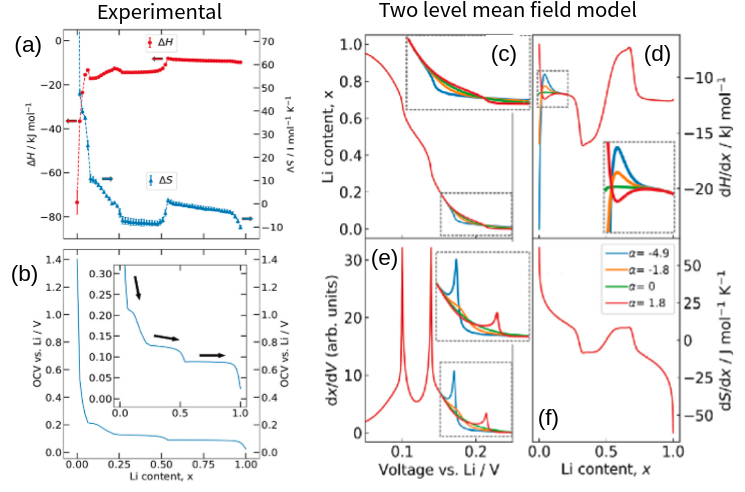
\includegraphics[scale=2]{figures/graphite_meanfield_alpha.png}
%    \caption{(a) experimental partial molar enthalpy and entropy profiles obtained during galvanostatic discharge of Li/graphite coin cells. (b) Experimental OCV. Mean field simulations of thermodynamic profiles: (c) Simulated OCV, (d) partial molar enthalpy, (e) dQ/dV (or voltammogram) (f) partial molar entropy. Results are shown dependent on different correction amplitudes, $\alpha$.  Reproduced from Ref. \citenum{Mercer2019}}
%    \label{fig:graphite_meanfield}
%\end{figure}
%\begin{itemize}
%    \item configuration entropy
%    \item electronic behaviour, link to dilute Li transitions ref. \citenum{Mercer2019}. Lack of implications for measureable entropy.
%\end{itemize}

\subsubsection{Ion diffusion in Li-GICs (Rana/Mike)} 
\label{sec:anodes_ion_diffusion}
% Hope to be ready by 27th November
% Mike to add one paragraph at the end. Just the diffusion coeffient part.
%(n = 1, 2) such as  LiC$_6$, stacking st-LiC$_6$, and LiC$_{12}$
% Introductory statement about kinetics.

Having outlined the use of atomistic techniques to evaluate observable thermodynamic properties of anodes, and in particular graphite, this section focuses on the computation of bulk dynamic properties by DFT and kinetic Monte Carlo (kMC) approaches.   

Li diffusivity is similar for stage I and stage II Li-GICs, \cite{persson2010} with the probable Li migration pathways for LiC$_{6n}$ illustrated in Figure~\ref{fig:Rl}.  \cite{RanaLiC6} These pathways were determined from DFT calculations within a climbing-image nudged elastic band (CI-NEB) approach. Here Li diffusion across the graphite layers through a carbon hexagon hollow (H) are denoted as the through-plane pathway. The in-plane or two-dimensional Li migration along the crystallographic ab plane occurs either by bridge (B) migration pathway where Li passes through a rectangle of carbon atoms of subsequent layers or top (T) migration pathway where Li passes in between two congruent carbon atoms.   

\begin{figure}
    \centering           
    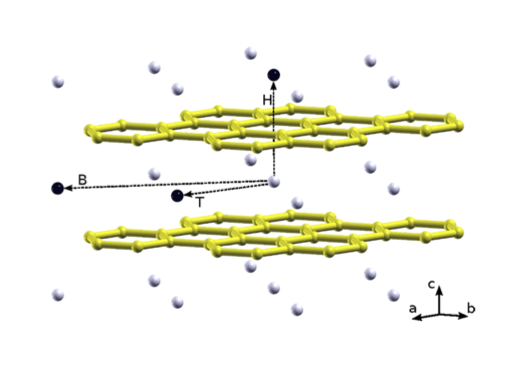
\includegraphics[scale=0.8]{figures/Islam-Fig-LiC6.png}
    \caption{Li migration pathway in LiC$_{6}$. In the through-plane pathway, lithium migrates through a carbon hexagon hollow (H) along the crystallographic c direction. The in-plane pathways are denoted as bridge (B) and top (T) reproduced with permission from ref.~\citenum{RanaLiC6}.}
    \label{fig:Rl}
\end{figure}
        
%We have performed various kinds of ion diffusion mechanisms.i.e, Li ion diffusion through a carbon hexagonal hollow (H) pathway which is denoted as the migration along c direction and in plane migrations as denoted as bridge (B) and top (T) migration pathways ref. \citenum{RanaLiC6}. 

 diffusion in the aforementioned through-plane pathways and in-plane pathways via the Frenkel and vacancy mechanisms, respectively, \citeauthor{RanaLiC6} showed that Li diffusion along the crystallographic c direction is kinetically prohibited due to a large activation energy barrier. \cite{RanaLiC6} The calculated activation energy for this migration pathway is extremely high (8.00 -- 8.23 eV), therefore, the Boltzmann probability for diffusion through pristine graphene planes is negligible at $T=300$ K. It is therefore likely that diffusion in the c direction occurs via grain boundaries \cite{persson2010lithium}. In contrast, the activation energy for Li diffusion in the ab plane is much lower (0.42 -- 0.52 eV), showing that in Li-GICs, Li diffuses mostly within the intercalation layers \cite{RanaLiC6}. Widely in literature, DFT based theoretical investigations provide the same qualitative trends for ion diffusion mechanisms in Li-GICs, the calculated activation barriers, however, vary slightly but are within the same order of magnitude. \cite{Imai-JAC-2007,persson2010lithium,Toyoura-JPCC-2010,Wang-RSC-Adv-2015} 

In order to gain insights into the Li diffusion process in graphite, far from equilibrium and under fast charging conditions, \citeauthor{Hakim} simulated a range of compositions between stage I and IV, i.e. dilute Stage I. \cite{Hakim} Their study determined reduced activation barriers in the in-plane migration pathways (0.2 -- 0.32 eV), which is attributed to the presence of a higher number of electrons compared to Li$^{+}$ ions, occurring at the very beginning of the lithiation cycle during fast charging conditions. This extra charge increases the interlayer spacing in the diffusion layer and adjacent channels, increasing the Li diffusivity \cite{Hakim}. \citeauthor{JI201866} investigated the anisotropic strain effects on lithium diffusion in graphite anodes using \textit{First Principles} DFT and kMC simulations. \cite{JI201866} According to their study, the activation energy for Li diffusion in unstrained Li$_{x}$C$_{6n}$ is 0.48 eV. The tensile strain along the direction perpendicular to the graphite planes facilitates in-plane Li diffusion by reducing the energy barrier and vice versa \cite{JI201866}. 

\citeauthor{gavilan-arriazu_kinetic_2020} have recently simulated the dynamic properties of lithium intercalation in graphite using kMC techniques \cite{gavilan-arriazu_kinetic_2020,gavilan-arriazu_effect_2020,GAVILANARRIAZU2018133}. These models considered exchange of Li with the the solution on one side of a slab (Figure~\ref{fig:graphite_kmcscheme}), with only interplanar Li transport allowed based on the diffusion barrier arguments presented above. Energetic barriers for Li exchange into/out of the graphite were calculated assuming Butler-Volmer kinetics based on experimental exchange current density data, while interplanar diffusion barriers were computed using random walk theory based on experimental data in the dilute limit. Respective barriers of 0.655 eV and 0.370 eV for exchange and interplanar diffusion were obtained. This approach enabled the simulation of several different dynamic properties dependent of lithium concentration, $x$, \cite{gavilan-arriazu_kinetic_2020,gavilan-arriazu_kinetic_2020} sweep direction \cite{gavilan-arriazu_kinetic_2020}, and temperature \cite{gavilan-arriazu_effect_2020}, with a few of these highlighted in Figure~\ref{fig:graphite_kmcobservables}. Additionally the importance of metastable Daumas-H\'{e}rold orderings in Stage II configurations \cite{GAVILANARRIAZU2018133} and clogging of lithium at the interface \cite{gavilan-arriazu_kinetic_2020} leading to slow Li insertion kinetics were identified as important challenges limiting the kinetics of the lithium (de)insertion processes.  


%\subsubsection{kMC approaches to Li-graphite} % Removed as it will likely be covered by Ezequiel Leiva in his review.
%\label{sec:anodes_kmc}
%-lead: Mike

%- lead: Mike + Rana
%- review: Chao/Denis



\begin{figure}
    \centering
    \includegraphics[scale=2]{figures/kmc_scheme.png}
    \caption{Representation of insertion and diffusion of lithium in graphite in kMC model.  From \citenum{gavilan-arriazu_effect_2020}}
    \label{fig:graphite_kmcscheme}
\end{figure}

\begin{figure}
    \centering
    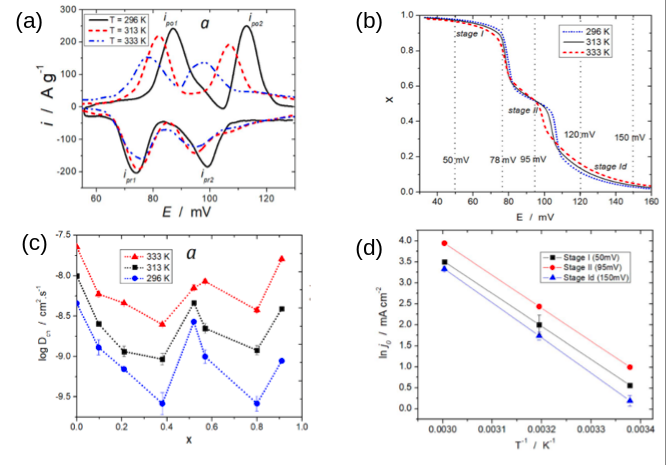
\includegraphics[scale=2]{figures/kmc_observables.png}
    \caption{Effect of temperature on dynamic behaviour of lithium insertion in graphite. (a) voltammograms (b) voltage profiles (isotherms) (c) diffusion coefficients, (d) exchange current density. insertion and diffusion of lithium in graphite in kMC model.  From \citenum{gavilan-arriazu_effect_2020}}
    \label{fig:graphite_kmcobservables}
\end{figure}


Having described modelling of the thermodynamics and bulk Li diffusion in graphite, the following section will focus on another important aspect for a multi-scale model: the structure and dynamics of the graphite edges.


\subsection{Graphite Surfaces and Interfaces (Arihant/Chao/Rana)}
\label{sec:anodes_surfaces_interfaces}

\subsubsection{Possible graphite surfaces and their stability}
% Chao and Rana to discuss online
% Estimated timeframe: 4th December
% lead: Rana + separate outlook to be merged later + Chao revision

As discussed above, investigating the bulk properties of lithium is of importance to understand the Li intercalation kinetics and charging/discharing rates in graphite. However, Li exchange occurs between the graphite surfaces and the electrolyte, hence a multi-scale model additionally needs to include these phenomena. Addressing the surface properties of graphite would improve the understanding of charging/discharging behaviours at graphite anodes and possibly enhance the charging/discharging rates.

As shown in Figure~\ref{fig:graphite_surfs} and section~\ref{sec:anode_bulk}, graphite consists of multiple stacked graphene layers. One of the exposed surfaces is the basal plane or the (001) surface, which has been widely investigated in both the theoretical and experimental studies.\cite{RanaLiC6,persson2010,toyoura2010effects,yao2012diffusion,nuli2006intercalation} In contrast, the non-basal planes attract less attention due to their complicated edge morphology. Recently, experimental studies characterised the SEI formation and growth along the graphite edges as opposed to the basal plane, \cite{liu2019situ,zhang2020operando} indicating the importance of the graphite non-basal plane in terms of Li intercalation.

\begin{figure}
    \centering
    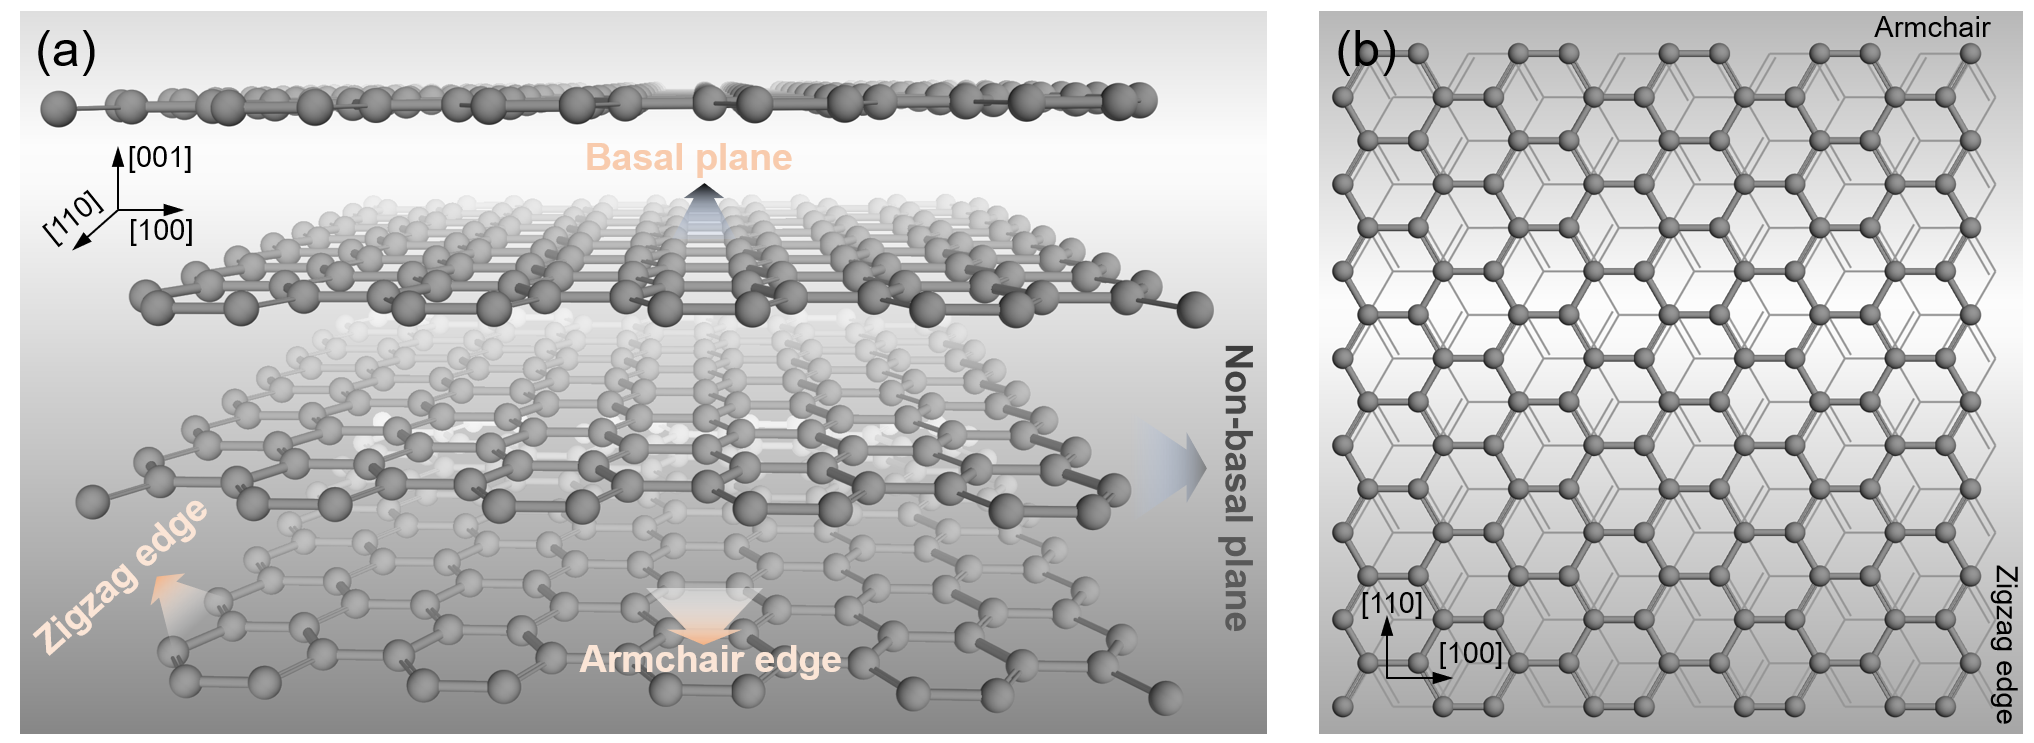
\includegraphics[scale=0.4]{figures/Graphite_surfs.png}
    \caption{(a) structures of the basal plane and the non-basal plane of graphite. The latter plane consists of different edges of graphites such as armchair edge and zigzag edge. (b) topological geometries of graphite edges.}
    \label{fig:graphite_surfs}
\end{figure}

\citeauthor{Rana-Graphite-Surf} investigated the stability of various low index graphite surface planes including the (001), (110), and (100) planes. The calculations were performed using dispersion corrected DFT approaches.\cite{grimme2010consistent,grimme2011effect} The surface energies of these planes were found to go in the order (001) $<$ (110) $<$ (100), \cite{Rana-Graphite-Surf} indicating that the (001) surface (the basal plane) is the most energetically favourable. This plane, however, is relatively inert towards Li intercalation due to the high diffusion barrier required for Li to go through the carbon hexagon \cite{RanaLiC6,persson2010}, as highlighted in the previous section on ion diffusion in Li-GICs (sec~\ref{sec:anodes_ion_diffusion}. Li intercalation of graphite particles must therefore proceed either via defects in the (001) plane or via the non-basal planes.

The (100) surface consists of nanoribbons with a zigzag edge, whereas the (110) surface adopts an armchair conformation. The relatively unstable surface planes, such as the (100) plane, can be stabilised by various procedures including chemisorption of oxygen atoms.\cite{Rosanna} It was found that the oxygen functional groups can stabilise the graphite edges and is critical for the formation of the SEI layer near the edge, thereby preventing graphite exfoliation.\cite{bernardo2015influence} Investigating those non-basal planes and their effects on Li intercalation are therefore important and are addressed in the following section.

\subsubsection{Surface Effect on Intercalation Energy (Chao)} 
Understanding the nature of Li intercalation in graphite is important for optimisation of the anode material. As described above, Li intercalation in the bulk of graphite has been widely investigated.\cite{persson2010,toyoura2008first,toyoura2010effects,yao2012diffusion,thinius2014theoretical} However, experimental Li diffusivities in graphite have been reported ranging from $10^{-6}$ -- $10^{-14}$ cm$^2$/s.\cite{toyoura2010effects,takami1995structural,yang2004evaluation,yu1999determination} DFT calculations\cite{persson2010} based on bulk graphite, however, indicate that Li diffusion coefficients based on the AABB and AA stacked graphite are around 10$^{-7}$ cm$^2$/s and decrease slightly with increasing Li concentration.\cite{persson2010} The smaller range of the diffusion coefficients from theoretical modelling indicates that the investigation beyond the bulk properties of graphite is necessary. As described in section~\ref{sec:anodes_surfaces_interfaces}, the basal plane is relatively inert towards Li intercalation.\cite{persson2010lithium} The non-basal plane, consisting of different edge morphology, attracts more attention due to observations of Li intercalation and SEI growth.\cite{liu2019situ,zhang2020operando} \citeauthor{uthaisar2010edge} studied the Li adsorption and diffusion on the edged graphene system using DFT.\cite{uthaisar2010edge} The graphene edges were found to not only affect Li adsorption but also the diffusion coefficient. Narrower graphite nanoribbons showed faster delithiation behaviour than the larger sized graphene due to the topological effect of graphene edges. This highlights that an in-depth knowledge of interface effects is needed to understand Li intercalation rate and enable rational optimisation of the battery performance.

\begin{figure}
    \centering
    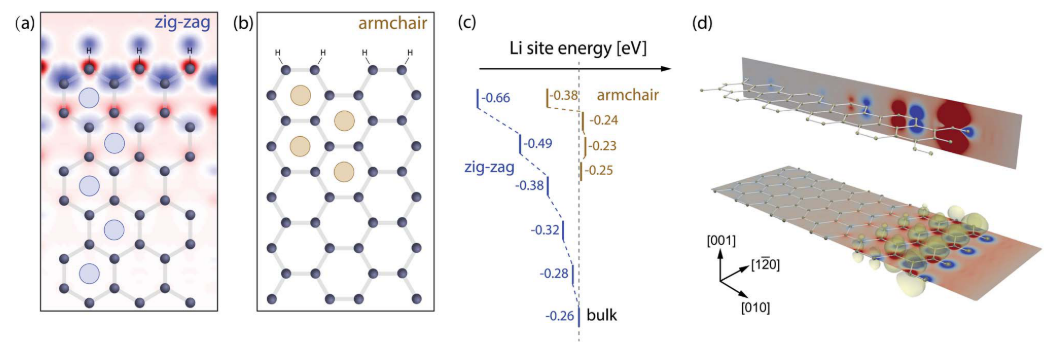
\includegraphics[scale=0.6]{figures/Intercalation energies.PNG}
    \caption{Structures of the zigzag-edged graphite (a) and the armchair-edged graphite (b). (c) shows the energy profile of Li adsorption in edged graphite. (d) is the spin densities of zigzag-edged graphite. The iso-surface value is 0.0002 e/\AA$^3$. Reproduced from Ref.~\citenum{peng2020lithium}}
    \label{fig:arm_zig}
\end{figure}

From an atomistic perspective, the surface and edge morphology of anode materials were found to have a strong impact on Li binding energies.\cite{uthaisar2010edge,leggesse2016lithium} Through investigating Si nano-structures, \citeauthor{chan2010controlling} found that Li has higher binding energies at the bulk site compared to the edge, requiring a higher energy cost of Li migration from the bulk towards the edge.\cite{chan2010controlling} In graphite anode materials, however, \citeauthor{leggesse2016lithium} reported that the edged graphite systems showed remarkably enhanced Li binding energies and high Li mobility along graphite edges.\cite{leggesse2016lithium} \citeauthor{peng2020lithium} recently quantified the edge effects on Li intercalation in graphite.\cite{peng2020lithium}. In their work, different edged graphites at dilute Li concentration were comprehensively investigated using DFT calculations. Interestingly, they found the unique topological electronic structures near the edges, particularly near the zigzag edge, induce distinct intercalation energies of Li in graphite. Figure~\ref{fig:arm_zig}c shows the Li adsorption energies at the armchair-edged and the zigzag-edged graphite, respectively. The adsorption energy, $E_{\rm{ads}}$, is expressed as:

\begin{equation}
E_{\rm{ads}} = E_{\rm{Li|Graphite}}-E_{\rm{Graphite}}-E_{\rm{Li}},
\label{eq:adsorption_energy}
\end{equation}

where $E_{\rm{Li|Graphite}}$, $E_{\rm{Graphite}}$, and $E_{\rm{Li}}$ are the energies of Li adsorption in graphite, the pristine graphite, and one Li in BCC Li metal, respectively. At the armchair edge, from the energy profile (cf. Figure~\ref{fig:arm_zig}), the adsorption energy of Li is the lowest at the edge site (-0.38 eV). With Li penetrating into the bulk, the adsorption energy decreases rapidly to -0.24 eV at the sub-surface site and becomes -0.26 eV at the bulk site. The topological geometry of the armchair edge promotes Li adsorption relative to the graphite bulk.

At the zigzag edge, the edge effect becomes even stronger due to the existence of the surface state at the edged carbons.\cite{fujita1996peculiar,lee2005magnetic} Figure \ref{fig:arm_zig}c shows that Li achieves a much lower adsorption energy of -0.66 eV at the zigzag-edge site, indicating the strong binding of Li at the edge. The edge effect in the zigzag system is much stronger than that at the armchair edge, and additionally penetrates into the bulk, indicated by the gradual decrease in magnitude of the Li adsorption energy from the edge to the bulk. 

The zigzag edge displays completely different spin densities contributed by the $p_z$ orbitals perpendicular to the graphene planes, as shown in Figure~\ref{fig:arm_zig}a-b. \cite{leggesse2016lithium,fujita1996peculiar,lee2005magnetic,peng2020lithium} These spin densities consist of the unpaired electrons accumulating on the edged carbons. The amplitude of this topological surface state gradually diminishes over a few bond distances beneath the surface. It is this surface state that interacts with Li at the zigzag edge and favours its adsorption. In summary, the graphite edges show stronger interactions with Li than those in the bulk. The effect is especially pronounced at the zigzag edge, which strongly stabilises Li binding due to the topological surface states.
    
\subsubsection{The Surface Effect on Li Diffusion (Chao)}
As Li obtains higher binding energies at the graphite edge due to the specific topological structure of graphite edges \cite{leggesse2016lithium,peng2020lithium}, it's worth examining the impact of those edges on Li diffusion. In bulk graphite, the diffusion barrier of Li jumping from one site to another is around 0.4 eV at the dilute limit.\cite{thinius2014theoretical} Li, however, exhibits completely different diffusion kinetics at graphite edges in contrast to those in the bulk.\cite{leggesse2016lithium,peng2020lithium} 

\citeauthor{peng2020lithium} show the energy profile of Li diffusion from the graphite edge towards the bulk at dilute Li concentration, figure \ref{fig:Li_diffusion_edge}. In the armchair-edged graphite, Li has to overcome an energy barrier of 0.43 eV to move from site 1 to site 2 and a 0.42 eV barrier to further move from site 2 to site 3. The direct jump from site 1 to site 3 has to overcome an energy barrier of 0.58 eV, and is therefore less favourable. In contrast, for bulk diffusion, Li needs to overcome a $\sim$0.43 eV barrier to move to either adjacent site. The higher diffusion barrier at the armchair edge is caused by the compensation of Li adsorption energy at the edge site. At the zigzag edge, Li obtains two different diffusion pathways. Li diffusion from the edge (site 1) to the subsurface (site 3), where the diffusion barrier is 0.48 eV. In contrast, there is only a 0.21 eV activation barrier for Li diffusion along the edge sites (site 1 to site 2), which is much lower. This indicates that Li is extremely mobile at the zigzag edge, which can be verified by the stronger flux connecting the edge sites compared to diffusion towards the bulk (cf. Figure \ref{fig:Li_diffusion_edge}). Due to the surface effect identified at the zigzag edge, Li favours diffusion along the edge direction within the first sub-surface sites as the diffusion barrier (0.41 eV) is still  lower than the barrier to moving Li into the bulk (0.49 eV). Markov chain analysis was conducted in \citeauthor{peng2020lithium}'s study to examine Li diffusion from the armchair edge and the zigzag edge to a bulk site 20 \AA \ below the edge surface (see Figure \ref{fig:Li_diffusion_edge}c). They demonstrated that Li diffusion from the armchair edge to the bulk site is around one order of magnitude faster than it diffusion from the zigzag edge to the bulk, due to the strong binding of Li at the zigzag edge that generates a deep potential well for Li.\cite{peng2020lithium}

On the basis of these studies, it was shown that the graphite edges have strong effects not only on the Li intercalation energies but also on its diffusion kinetics.\cite{leggesse2016lithium,peng2020lithium} The effect is pronounced at the zigzag edge.\cite{bernardo2015influence,velicky2019electrochemistry,gerischer1985interpretation} Thus much more sluggish (de)intercalation kinetics are expected at that edge compared to the armchair edge. Strategies including promoting growth of armchair edge over zigzag edge during synthesis of graphite nanomaterials and tuning the edge properties by chemical doping to improve Li diffusion rate towards the bulk could be useful to enhance Li (dis)charging rate for graphite anodes.\cite{weydanz1994behavior,way1994effect,endo2001scanning} These studies can also offer some universal thoughts for investigating the interface effects of other materials such as the cathode, from the atomistic perspective. Prior to Li intercalation into graphite, the Li desolvation process is also an important step affecting the overall charging/discharging rate. However, due to the complicated solid-liquid interface, addressing the graphite interaction with the electrolyte is an extremely challenging aspect for both modelling and experiment, as discussed in the following section.

\begin{figure}
    \centering
    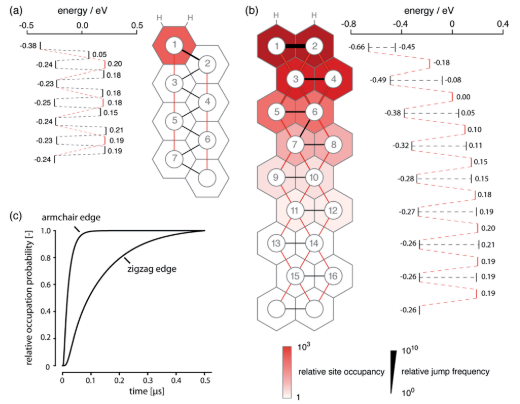
\includegraphics[scale=0.5]{figures/Graphite_edge_effects.PNG}
    \caption{Li diffusion at (a) the armchair-edged and (b) the zigzag-edged graphite. The hexagons indicate lattice site and the colours show occupancy probability relative to that in the bulk. The width of the lines connecting sites implies the jump frequencies. (c) shows the occupation probability for Li to occupy a site approximately 20 \AA \ below the graphite edge relative to the steady-state value after being introduced at time zero at the edge. Reproduced from Ref.\citenum{peng2020lithium}}
    \label{fig:Li_diffusion_edge}
\end{figure}

\subsubsection{Solid-Electrolyte Interphase (SEI)}
The Solid-Electrolyte Interphase is an important component of the rechargeable Li-ion battery, which is formed from the decomposition of the electrolyte and solvent and their deposition on the anode surface. The SEI allows transport of Li$^+$ ions but blocks the transfer of electrons, thereby stopping further electrolyte decomposition reactions.\cite{Winter2009, VERMA20106332} Here we discuss aspects of the SEI related to our discussion of Li-ion diffusion energy barrier in bulk and graphite surfaces. A recent comprehensive review on the atomistic modelling of the SEI describes several other aspects of the SEI in detail:\cite{Wang2018} 
\begin{itemize}
    \item Electrolyte and solvent reduction mechanisms, including: prediction of the reduction voltage for each solvent and electrolyte species, the effect of the electrolyte solvation structure,the effect of anode surface termination, and the dynamic buildup of the nanometer thick SEI layer
    \item Modification of the SEI by electrolyte additives and prediction of new electrolyte additives 
    \item Correlation of the SEI properties with battery performance, including: the electron insulating properties of the inorganic components in the SEI, the ionic conductivity of the SEI components, Li-ion desolvation at the SEI/electrolyte interface, chemical stability of the SEI components, and mechanisms of SEI growth and battery aging
    \item The use of coatings to artificially design the SEI
\end{itemize}

One of the ways of describing the SEI is via the implicit continuum models described in sec.~\ref{sec:dft+cont}. Applying their DFT + implicit electrolyte model, on an armchair edge of 1634-atom graphite slab in contact with a 0.5 M LiPF$_6$/EC solution, \citeauthor{Dziedzic2020} calculated that a Li atom is 2.34 eV more stable at the graphite edge than in the electrolyte solution.\cite{Dziedzic2020} Similarly, \citeauthor{haruyama2018} found favourable energetics for Li intercalation from the electrolyte solution into the graphite edge.\cite{haruyama2018} They also studied the variation in energy as a function of Li distance from the graphite edge, as shown in figure \ref{fig:gel}. In \citeauthor{haruyama2018}'s model, Li intercalation is accompanied by an electron gain from the external circuit. This was implemented using a grand canonical version of electronic DFT, where the number of electrons in the electrode can change subject to fixed electrode potential. Correspondingly, the appropriate thermodynamic quantity to represent this ensemble is the grand potential, $\Omega=A-\mu_e N_e$, which is plotted on the y axis for several different constant chemical potentials of electrons, $\mu_e$. Two illustrative cases include: (a) the potential of zero charge (PZC), which is the electrochemical potential of a charge-neutral Li-graphite system, and (b) the equilibrium potential (c.f.  sections~\ref{sec:properties_equilibriumvoltage} and ~\ref{sec:anodes_ocv}), where the net change in the grand potential for the intercalation reaction becomes zero. \citeauthor{haruyama2018}'s simulations estimate an energy barrier of around 0.6 eV for Li intercalation into the graphite edge, which is close to the experimental measurements using impedance spectroscopy,\cite{Yamada2009}
\begin{figure}
    \centering
    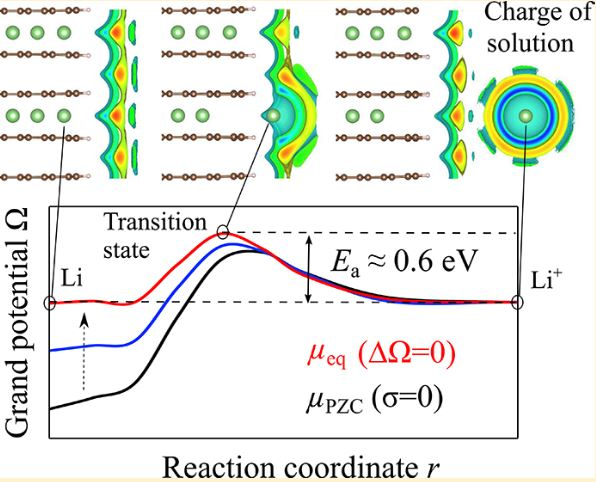
\includegraphics[scale=0.6]{figures/graphite-interface.JPG}
    \caption{Profiles of grand potential $\Omega$ as a function of the Li-position during Li-intercalation process at the interface between graphite edge and an implicit electrolyte solution. The simulation is performed at conditions of constant chemical potential of electrons $\mu_e$ (constant electrode potentials similar to experiments). Reproduced from Ref. \citenum{haruyama2018}}
    \label{fig:gel}
\end{figure}

Another way to describe the SEI is via explicit consideration of SEI components. \citeauthor{Shi2012} performed a direct calculation of Li-ion transport in the Li$_2$CO$_3$ component of the SEI,\cite{Shi2012} via DFT-based climbing image NEB calculations (section \ref{sec:methods_neb}). Two mechanisms for Li$^+$ diffusion were considered, namely, the knock-off and direct hopping mechanisms, which were found to have energy barriers of 0.31 eV and 0.54 eV respectively, as shown in figure \ref{fig:sei}. The Li self-diffusion coefficient was calculated to be $1.1\times10^{-7}$ cm$^2$/s and $8.4\times10^{-12}$ cm$^2$/s respectively. Estimating the formation energy of corresponding defects in the lattice of Li$_2$CO$_3$ as a function of voltage, the total activation energy barrier for Li-ion diffusion was predicted to be in the 0.67-1.07 eV range for the knock-off mechanism and between the 0.92-1.32 eV range for the direct-hopping mechanism.
\begin{figure}
    \centering
    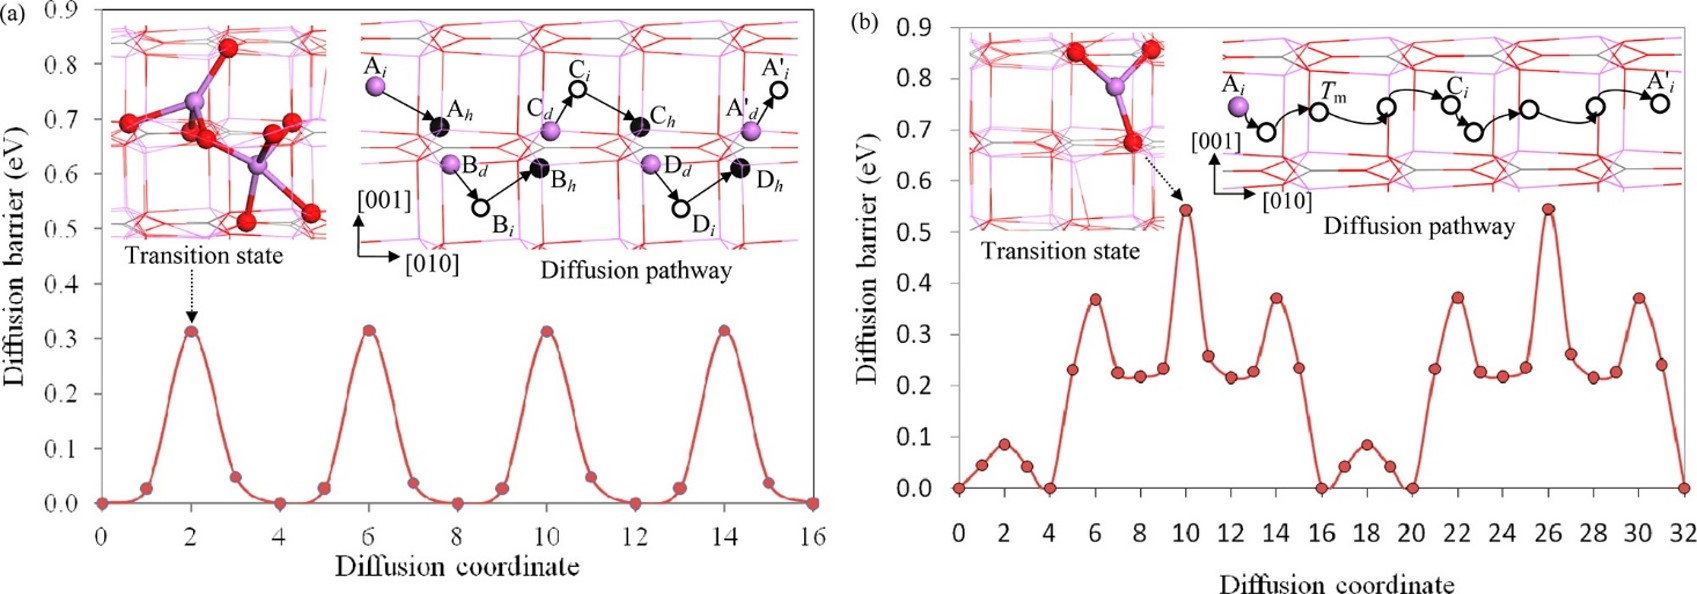
\includegraphics[scale=0.5]{figures/sei.jpg}
    \caption{Energy barrier for Li-ion transport in the SEI via (a) knock-off (b) direct hopping mechanisms. Reproduced from Ref. $\citenum{Shi2012}$}
    \label{fig:sei}
\end{figure}

The predicted values of Li-ion diffusion energy barrier by both the implicit model and the explicit models described above are significantly higher than that in the bulk of graphite, which is reported to be between 0.2-0.5 eV (cf. section~\ref{sec:anodes_ion_diffusion}).\cite{thinius2014theoretical, RanaLiC6, Hakim, persson2010} This indicates a limiting role of the SEI in determining overall kinetics of Li-ion diffusion and the overall rate-capability of Li-ion batteries.

\subsection{Outlook and challenges for anodes}

We here highlight the following outstanding challenges regarding atomistic modelling in anodes.
    % Big challenges:
    % Small challenges:
    % Outlook:
\begin{itemize}
    \item Many aspects of modelling the bulk behaviour of lithium (de)insertion graphite are well understood by now. However, there are outstanding challenges regarding the role of metastable phases in the kinetics of staging behaviour. In particular, new theoretical frameworks need to be developed to be able to understand, more generally, the connectivity between different phases and the effect of this on measurable behaviour like the OCV.
    \item An additional point is the role of entropy effects and in particular the role of the configurational entropy of lithium insertion. Longer length scales, i.e. continuum models, still assume that the entropy follows an ideal solid solution behaviour. One promising link would be to use the results from Monte Carlo calculations to parameterise a phase field model and in this way more accurately describe entropy effects.
    \item The quantitative accuracy of DFT predictions is limited by the accuracy of the description of the van der Waals interactions. Better descriptions of these interactions may shed light on the description of the dilute stages of order $>$ II.

    \item Arihant: modelling surface and interface effects: moving beyond a Butler-Volmer description
    \begin{itemize}
        \item the current models of the interface are too simplistic or represent an ideal situation instead of dealing with the complexity / reality of the SEI.
        \item systematic coarse-graining approach involving multi-length-scale and multi-time-scale physics can help in understanding the complex nature of the SEI and its influence on performance of Li-ion batteries.
        \item Controlling and improving the properties of SEI is crucial to improve the overall rate capability of Li-ion batteries, as interface seems to be the bottleneck for Li-ion diffusion.
    \end{itemize}
    \item The section focused on graphite, the predominant anode material in present-day lithium ion cells. From a materials design perspective, one can use the results of atomistic modelling to predict modifications to graphite that could enhance its capacity, durability or rate performance. This could include: systematic modifications to the edge morphology or the use of dopants, as described above, or tuning of the interlayer spacing.
%Rana%
    \item To achieve increased energy densities, the intercalation chemistry of graphite must be replaced by anode materials that are capable of electrochemically alloying with lithium. Silicon, due to its high gravimetric capacity of 4200 mAh g$^{−1}$ upon full lithiation with the formation of Li$_{22}$Si$_5$, has achieved tremendous attention as an anode material. Silicon possesses other desirable qualities, such as it has a low electrochemical potential between 0.37 and 0.45 V versus Li/Li$^+$, which is 0.27 V higher than graphite. Therefore Si anode can contribute to high working voltage when paired with a cathode, leading to a high energy density in a full LIB. Si, being the second most abundant element in the Earth’s crust, is very cost effective. Additionally, due to its good environmental compatibility, low toxicity, and relatively stable chemical property compared to graphite, Si has become a very promising candidate for next-generation Li battery anodes. 
    
    The phase diagram of lithium and silicon shows five crystalline intermetallic Zintl-like phases: Li$_{21}$Si$_{5}$, Li$_{13}$Si$_{4}$, Li$_{7}$Si$_{3}$, Li$_{12}$Si$_{7}$, and LiSi. A metastable crystalline phase with the composition Li$_{15}$Si$_{4}$ and amorphous Li$_x$Si$_y$ also exist. The crystalline phases tend to be more kinetically stable than the corresponding amorphous phases due to their lower formation energy. 
    
    In spite of the technological significance of Si and Li-Si-based anodes, data on the Li diffusion in those materials are still eluding. Multi-scale modelling can be utilized to get insight into this aspect as it was done for graphite and LIGICs compounds.
    
    One inevitable challenge with Si and all other alloy-type anode materials, is their poor cycling stability during charge and discharge. Upon full lithiation, the volume of Si can expand to more than three times of its original value which poses a real challenge for Si electrodes to retain its morphology over cycling. In order to get rid of this problem, several technologies have been proposed to improve the morphology including development of different Si robust nanostructures (0D nanoparticles (NPs), hollow NPs, 1D nanowires, 2D film-like Si, and 3D Si structures), development of composites (Si/carbon composites, Si/polymer composites, Si alloys, and Si/metal oxide composites) etc. Multi-scale modelling approaches could be strong tools to analyse these technologies and propose improved materials as anodes compared to the existing ones.   
    
    
    
    \item atomistic methods may also eventually lead to better materials, such as silicides. One could also explore modifications to existing materials like lithium titanate (LTO), including recent promising work on lithium niobium titanate. 
    
    
\end{itemize}

\end{document}